\chapter{Die Enigma-Maschine}\label{ch:die-enigma}
\section{Einführung}\label{sec:einfuhrung}

Um die Funktionsweise der Turing-Welchman-Bombe und ihrer Software-Nachbildung zu verstehen, muss zuerst die Enigma-Maschine verstanden werden.
Im Folgenden sei ein Überblick über die Enigma-Maschine gegeben.
Die Enigma-Maschine ist eine Rotor-Chiffrier\-maschine, die 1918 von Arthur Scherbius zum Patent angemeldet wurde und hauptsächlich im Zweiten Weltkrieg zum Einsatz kam.
Aufgrund der Sicherheitsanforderungen der deutschen Wehrmacht wurde die kommerziell erwerbliche Enigma-Maschine modifiziert.
In~\cref{fig:enigma_complete} ist eine solche modifizierte Enigma-Maschine zu sehen.
Die von der Wehrmacht eingesetzten Enigma-Maschinen verfügten zunächst über drei Walzen~(Ziffer~13).
Neuerungen waren das Steckerbrett~(siehe~\cref{fig:enigma_complete}~front) und gegen Ende des Krieges eine zusätzliche, vierte Walze. 
Adaptiert wurde die Umkehrwalze~(Ziffer~20).
Hier wird, wenn nicht ausdrücklich erwähnt, ausschließlich die Enigma M3 mit drei Walzen betrachtet.
\nopagebreak
\begin{figure}[htbp]
	\centering
	\includegraphics[width=.42\linewidth]{Enigma/Enigma-plakat}
	\caption{Die Enigma-Maschine (Foto Deutsches Museum München)}
	\label{fig:enigma_complete}
\end{figure}

\newpage

\section{Funktionsweise}\label{sec:funktionsweise}

\subsection{Walzen}\label{subsec:walzen}
Jede der von der Enigma-Maschine verwendeten Walzen besitzt eine interne Verdrahtung, welche eine monoalphabetische Substitution durchführt.
Das bedeutet, dass jeder Buchstabe auf genau einen anderen Buchstaben abgebildet wird.
In~\cref{fig:rot1_wiring} ist die Verdrahtung der Walze~I zu sehen.

\begin{figure}[htbp]
	\centering
	\caption{Verdrahtung Walze I}
	\resizebox{\textwidth}{!}{%
		\begin{tabular}{|c|c|c|c|c|c|c|c|c|c|c|c|c|c|c|c|c|c|c|c|c|c|c|c|c|c|}
			\hline
			A & B & C & D & E & F & G & H & I & J & K & L & M & N & O & P & Q & R & S & T & U & V & W & X & Y & Z\\
			\hline
			E & K & M & F & L & G & D & Q & V & Z & N & T & O & W & Y & H & X & U & S & P & A & I & B & R & C & J\\
			\hline
		\end{tabular}
	}
	\label{fig:rot1_wiring}
\end{figure}

Diese Verdrahtung ist starr und individuell für jede Walze.
Eine Enigma-Walze hat 26 Eingangs- und 26 Ausgangs-Kontakte.
Zudem kann eine Walze 26 Ausgangspositionen annehmen, jeweils repräsentativ für das Alphabet.
Wird nun an den Eingangskontakt \glqq A\grqq{} Spannung angelegt, so wird dieser Buchstabe durch die interne Verdrahtung zu einem \glqq E\grqq{} permutiert.

Um die Enigma-Maschine in Betrieb zu nehmen, müssen drei von acht möglichen Walzen ausgewählt werden.
Diese drei Walzen werden in Reihe geschaltet.
Die rechte Walze wird bei jedem Tastendruck um eine Position weitergerückt.
Hat diese Walze eine komplette Rotation vollzogen, rückt die Walze links neben ihr um eine Position weiter.\footnote{Eine Analogie hierfür ist das Verhalten eines mechanischen Kilometerzählers oder das Verhalten von Sekunden-, Minuten- und Studenzeigern einer Uhr.}
Die 26 Eingangs-Kontakte der rechten Walze werden durch 26 Kontakte der Enigma-Maschine versorgt, welche mit der Tastatur verbunden sind.
Die Enigma-Maschinen Kontakte sind starr und bewegen sich nicht.
Wird nun ein \glqq A\grqq{} betätigt, während sich die Walze in Stellung \glqq A\grqq{} befindet, wird diese zuerst rotiert und dann durchlaufen.
Der Strom nimmt somit den \glqq B\grqq{} Pfad.
Das Resultat dieser in Reihe geschalteten Walzen ist eine polyalphabetische Substitution.

\begin{figure}[htbp]
	\centering
	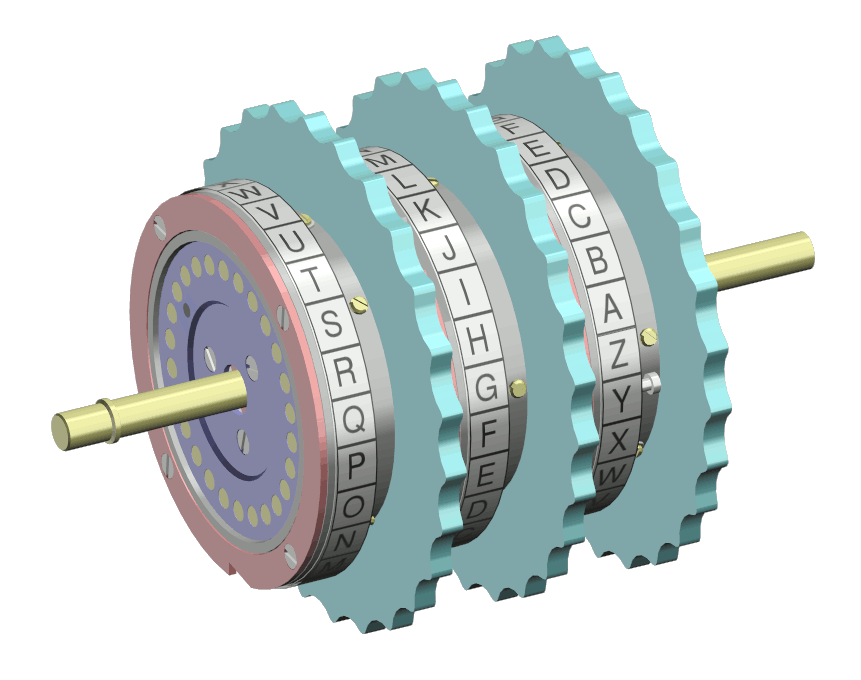
\includegraphics[width=.4\linewidth]{Enigma/Enigma-rotor-set}
	\caption{Enigma-Walzen\autocite{enigmarotorset2004}}
	\label{fig:enigma_rotors}
\end{figure}

Die Walzenstellung sagt aus, in welcher Ausgangsposition sich die Walzen befinden.
Diese kann durch ein Sichtfenster vom Bediener abgelesen werden.
Eine weitere Einstellmöglichkeit der Walzen ist die sogenannte Ringstellung.
Sie verändert die Relation der sichtbaren Buchstaben zu der internen Verdrahtung und bewegt die Übertragskerbe, %(siehe~\cref{fig:enigma-rotor-contact})
die festlegt, wann sich die Walze links von der aktuellen bewegt.
%Da die Ringstellung bei dem Entschlüsselungsverfahren der Turing-Bombe keine weitere Rolle spielt, wird hier nicht weiter darauf eingegangen.

%\begin{figure}[htbp]
%	\centering
%	\begin{tikzpicture}
%		\node at (0,0) {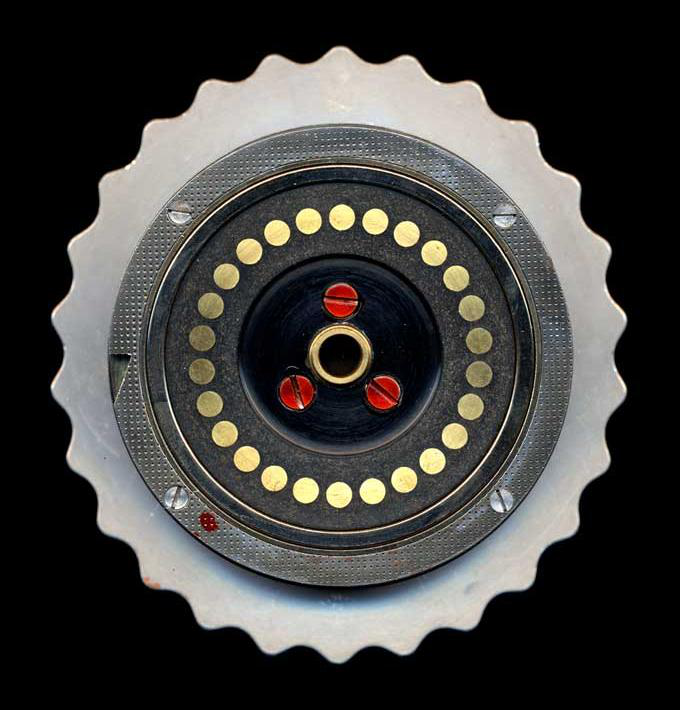
\includegraphics[width=.3\linewidth]{Enigma-rotor-flat-contacts.png}};
%		\draw[red, very thick, ->] (-3,-0.5) -- (-1.5,-0.1);
%		\node[red, anchor=west] at (-5,-0.8) {Übertragskerbe};
%	\end{tikzpicture}
%	\caption{Walzen Frontansicht mit Übertragskerbe}
%	\label{fig:enigma-rotor-contact}
%\end{figure}

\newpage
\subsection{Umkehrwalze}\label{subsec:umkehrwalze}
Der originalen Patentschrift\autocite{scherbiuschiffriermaschine1925} von 1918 ist zu entnehmen, dass sehr frühe Enigma-Maschinen nicht involutorisch wirkten.
%Das bedeutet ganz allgemein, dass $E_K \ne D_K$ ist.
%$E_K$ ist die Chiffrierfunktion in Abhängigkeit eines Schlüssels – hier die Konfiguration der Enigma-Maschine.
%$D_K$ stellt die Dechiffrierfunktion dar.
%Es wird also zur Dechiffrierung eine andere Funktion, als zur Chiffrierung benötigt.
Konkret bedeutet das für sehr frühe Enigma-Maschinen, dass diese zur Dechiffrierung einer Nachricht, die zuvor von einer Enigma-Maschine chiffriert wurde, einen speziellen Modus benötigen.
Um die chiffrierte Nachricht zu dechiffrieren, muss ein Hebel umgelegt werden und die Walzen müssen in Ausgangsstellung gebracht werden.
Nun wird Strom nicht von rechts nach links, sondern von links nach rechts durch die Walzen geleitet.

Da das daraus resultierende Gesamtgewicht von rund 50\si{\kg} unakzeptabel für den Feldeinsatz war und der zusätzlich benötigte Mechanismus fehleranfällig erschien, wurde die Umkehrwalze oder auch der Reflektor von der Wehrmacht adaptiert.
Die Umkehrwalze sorgt dafür, dass 
%$E_K = D_K$ ist, sprich 
mit der gleichen Einstellung und \glqq Modus\grqq{} ein beliebiger Text sowohl chiffriert als auch dechiffriert werden kann.
Wie in~\cref{fig:enigma_reflector} zu erkennen, besitzt die Umkehrwalze nicht 52, sondern nur 26 Kontakte.
Sie \glqq wirft\grqq{} das Signal zurück und schickt dieses ein weiteres Mal, in entgegengesetzter Richtung durch die Walzen.
Es werden Buchstabenpaare gebildet, welche die Umkehrwalze kommutativ wirken lassen und die Enigma-Maschine involutorisch machen.
Somit wurde sich die Komplikation und das Gewicht des Dechiffrierungs-Modus gespart.

\begin{figure}[htbp]
	\centering
	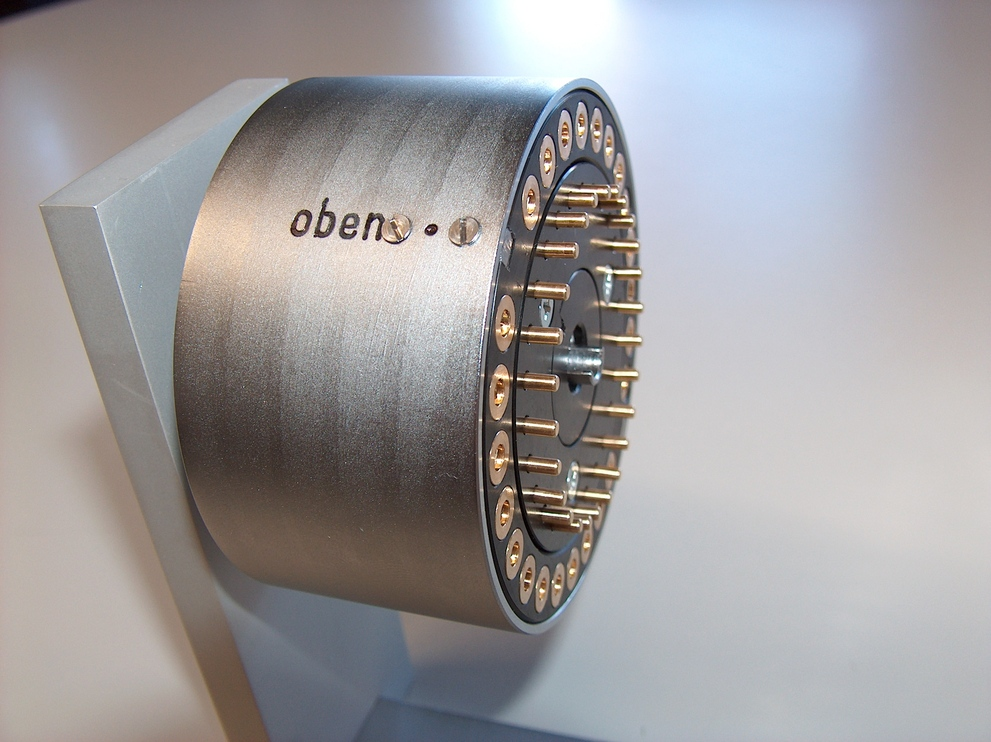
\includegraphics[width=.5\linewidth]{Enigma/UKW-D}
	\caption{Umkehrwalze-D Replika\autocite{enigmareflektor}}
	\label{fig:enigma_reflector}
\end{figure}

Doch leider ist dieser geniale Einfall die wohl größte Sicherheitslücke der Enigma.
Aufgrund der Buchstabenpaare wird niemals ein Buchstabe auf sich selber abgebildet.
Das Ergebnis ist eine sogenannte fixpunktfreie Permutation.
Kein Element behält somit seine Anfangsposition.
Da $\mathcal{A}\coloneqq\{\mathrm{A}, \mathrm{B}, \mathrm{C}, \ldots, \mathrm{Z}\},\; \forall x \in \mathcal{A}:\; E_K(x) \ne x$ bleiben nur noch wenige Positionen übrig, an welchen sich ein bekannter Funkspruch-Abschnitt (Known-plaintext) befinden kann.

%\newpage

\subsection{Steckerbrett}\label{subsec:steckerbrett}

Da ein Schlüsselraum von 686.518.560 Möglichkeiten\footnote{Diese Berechnung berücksichtigt die Anomalie des Fortschaltmechanismus.\autocite{wiki:enigma}} der Wehrmacht nicht genügte, wurde der Enigma-Maschine das Steckerbrett hinzugefügt.
Das Steckerbrett wirkt kommutativ und substituiert zwei Buchstaben. 
Es wird jeweils vor und nach dem Walzensatz traversiert. 
Die Anzahl von 150.738.274.937.250\autocite{wiki:enigma} zusätzlichen Möglichkeiten durch das Steckerbrett erscheint gewaltig, jedoch werden all diese Möglichkeiten von der Turing-Welchman-Bombe überwunden und spielen für die Sicherheit der Maschine de facto keine Rolle.

\begin{figure}[htbp]
	\centering
	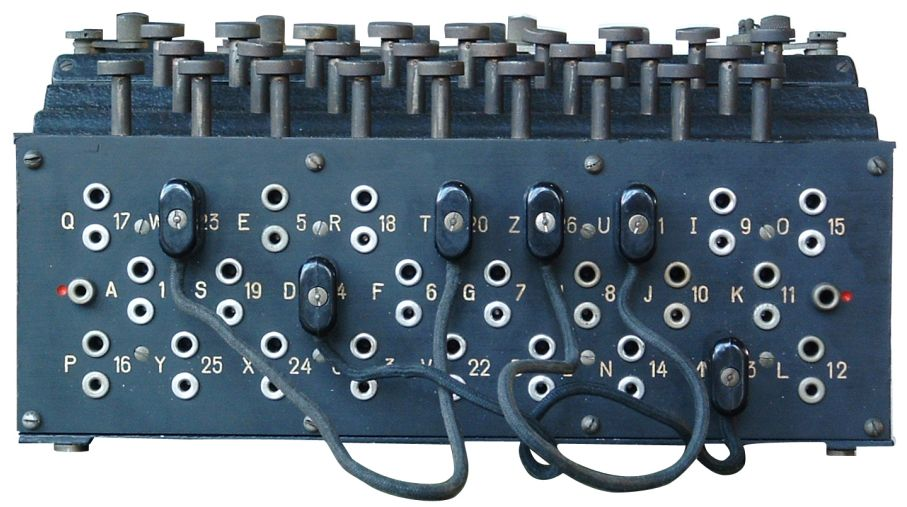
\includegraphics[width=.4\linewidth]{Enigma/enigma-steckerbrett}
	\caption{Enigma-Steckerbrett\autocite{wiki:enigmasteckerbrett}}
	\label{fig:enigma_plugboard}
\end{figure}

Die Permutation der Buchstaben lässt sich durch folgende Formel beschrieben:
%TODO Enigma Einstellung in Unterfunktionen?
\fmbox{\textbf{Permutation der Buchstaben}
	\[
	E_K: \mathcal{A} \longmapsto \mathcal{A},\quad E_K(x) \coloneqq S\circ W_1^{-1} \circ W_2^{-1} \circ W_3^{-1} \circ U \circ W_3 \circ W_2 \circ W_1 \circ S(x)
	\]
}

\section{Übertragung der Nachrichten}\label{sec:uebertragung-der-nachrichten}
Bei der Enigma-Maschine wurde jeden Tag ein Tagesschlüssel eingestellt, welcher durch ein Code-Buch vorgegeben war.
Dieser Tagesschlüssel bestand darin, welche drei der acht Walzen der Schlüssler in welcher Reihenfolge einzusetzen hatte, welche Ringstellung und welche Steckerbrett-Verbindungen für den Tag gültig waren.
Von 13 möglichen Steckerbrett-Verbindungen wurden meistens 10 vorgegeben.
In~\cref{fig:enigma_code_book} ist ein Code-Buch-Auszug für eine Enigma-Maschine mit einer veränderlichen Umkehrwalze (UKW-D) zu sehen.

\begin{figure}[htbp]
	\centering
	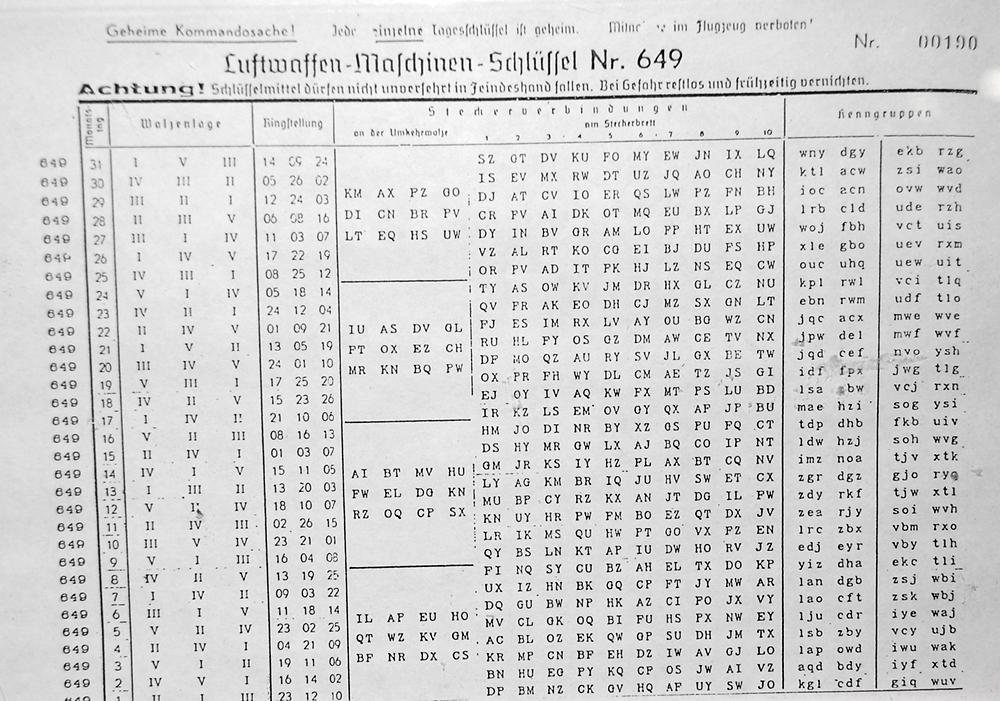
\includegraphics[width=.6\linewidth]{Enigma/Enigma-code-book}
	\caption{Code-Buch-Auszug\autocite{wiki:enigmacodebook}}
	\label{fig:enigma_code_book}
\end{figure}

\newpage

Nach 1938 musste der Schlüssler sich eine eigene Grundstellung der Walzen überlegen, mit welchem er den sogenannten Spruchschlüssel verschlüsselte.
Nun überlegte sich der Schlüssler einen \glqq zufälligen\grqq{} Spruchschlüssel, mit dem der Text chiffriert wurde.\footnote{In Wahrheit wählten die Schlüssler oft den gleichen Schlüssel, der meist persönliche Informationen wie zum Beispiel den Namen der Freundin enthielt.}
Dieser Spruchschlüssel gibt die Walzenstellung für die folgende Nachricht an.
Der \glqq zufällige\grqq{} Spruchschlüssel wurde mit der Grundstellung verschlüsselt und ergab zusammen mit der Grundstellung und anderen Zusatzinformationen den \glqq Spruchkopf\grqq.
Dieser Spruchkopf wurde dann im Klartext an den Empfänger übertragen.  
Da jedoch die Ringstellung die Relationen der sichtbaren Buchstaben zu der internen Verdrahtung ändert, war die Information der Grundstellung und des Spruchschlüssels für die Alliierten nicht wirklich brisant.
Der Schlüssler gab den zu verschlüsselnden Text nach bestimmten Regeln ein\autocite{schluesselm1940}: Eigennamen wurden verdoppelt, Satzzeichen wie ein Punkt wurden durch ein X ersetzt, Uhrzeiten wurden ausgeschrieben und viele mehr.

Der Empfänger musste nun auf seiner Enigma-Maschine den Tagesschlüssel einstellen und die Walzen in die über den Spruchkopf mitgeteilte Grundstellung bringen.
Nun entschlüsselte er mit dieser Einstellung den Spruchschlüssel.
Wenn die Walzenstellung mitgeteilt durch den entschlüsselten Spruchschlüssel auf der Enigma-Maschine eingestellt wurde, konnte die eigentliche Nachricht dechiffriert werden.
In~Anhang~\ref{ch:msg-trans} ist der Vorgang einer Nachrichtenübertragung zu sehen.
Hierbei stellt $K_S$ den Spruchschlüssel und $K_T$ den Tageschlüssel dar.

Hierbei sei angemerkt, dass sich das Verfahren der Nachrichtenübertragung über die Kriegsjahre mehrfach änderte.
So war die Grundstellung der Walzen vor 1938 noch Teil des Code-Buchs.

